\documentclass[12pt,a4paper]{article}
\usepackage{graphicx, booktabs, siunitx, amsmath, geometry, float}
\usepackage{subcaption}
\geometry{margin=2.5cm}
\title{XXX}
\author{Gregorio Jaca U8L9B9, Peter Tallosy K14WR1 }
\date{\today}

\begin{document}
\maketitle

% Abstract
\begin{abstract}

    Sensitive light polarization allows us to characterize the optical properties of different samples.
    We measured the optical retardation of a voltage controlled liquid cristal (LC) cell. We built a setup which allows us to measure the linear dichroism in hemozoid in suspension, a malaria indicator. Using samples of known concentration, we constructed a calibration curve which allows us to quantify the concentration of an unknown sample.

\end{abstract}

% Introduction
\section{Introduction}

Molecules with anisotropic shapes can have anisotropic orientation-dependent optical effects individually. In most cases, aggrgates of randomly oriented molecules have no net anisotropic effect. Liquid crystal (LC) phases at the boundary of a liquid and a solid crystal with an ordered orientation, which can controlled by an electric field. Taking advantage of this propery, we use a LC cell with a volatge controlled waveplate which generates the alternating electric field, which acts as a voltage-controlled waveplate.


\section{Results and Discussion}

\subsection{Basic characterization of film polarizers}

% TASK 1

We measure the analyzer orientation dependence of the intensity. We considering the room background lighting by registering the measured intensity when the laser was off, and considering that the baseline.

\begin{figure} [H]
    \centering
    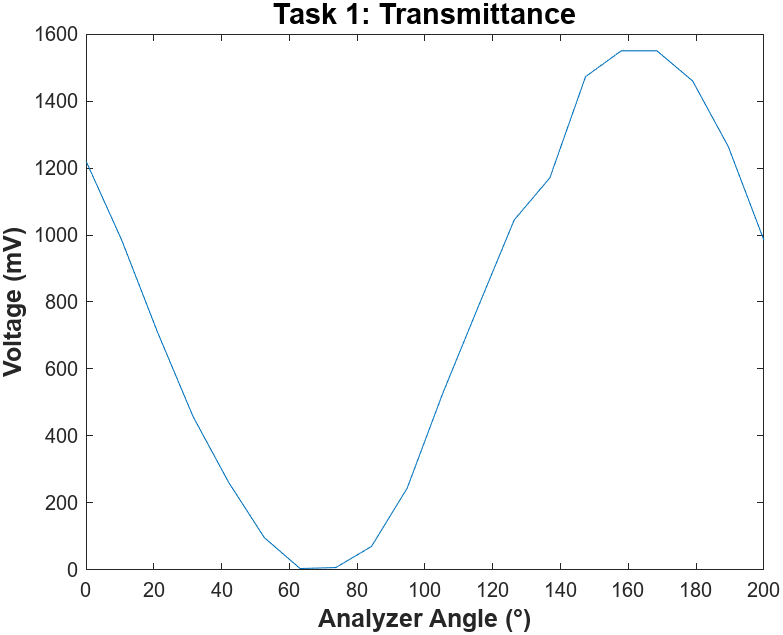
\includegraphics[width=0.35\linewidth]{figs/task1_transmittance.png}
    \caption{Light intensity dependency on analyzer orientation.}
    \label{fig:t1}
\end{figure}

The data shows a $I \sim \cos^2\varphi$ dependency of the light intensity with the polarizer angle. The extintion ratio = \frac{I_\perp}{I_\parallel} quantifies the quality of a polarizer, with a smaller value indicating a higher quality, was calculated and we obtained a value of 0.0026. This measurement allowed us to determine the polarization direction of the light source.


\subsection{Liquid crystal cell}

% TASK 2
 The optical path has a two orthogonal linear polarizers with the LC in the middle. If the LC cell was not there, there would be practically no light at the detector. The LC cell, when spanning an angle of 45° circularly polarizes the light. In practice we determined the angle by LC cell until we obtained a maximum intensity at the detector, which corresponds to the configuration where the incoming light is circularly polarized the most. This was achieved by rotating the LC cell approximately 50°. The analyzer linear polarizer should have no effect on the circularly polarized light, which implies that the measured intensity should not depend on the analyzer's angle. This would make a circular polar plot.

\begin{figure}[H]
    \centering
    \begin{subfigure}{\linewidth}
        \centering
    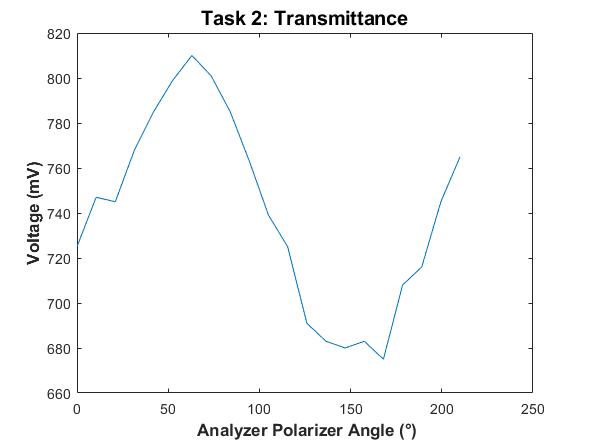
\includegraphics[width=0.35\linewidth]{figs/task2_transmittance.png}
    \end{subfigure}
    
    \vspace{1em} % 

    \begin{subfigure}{\linewidth}
        \centering
    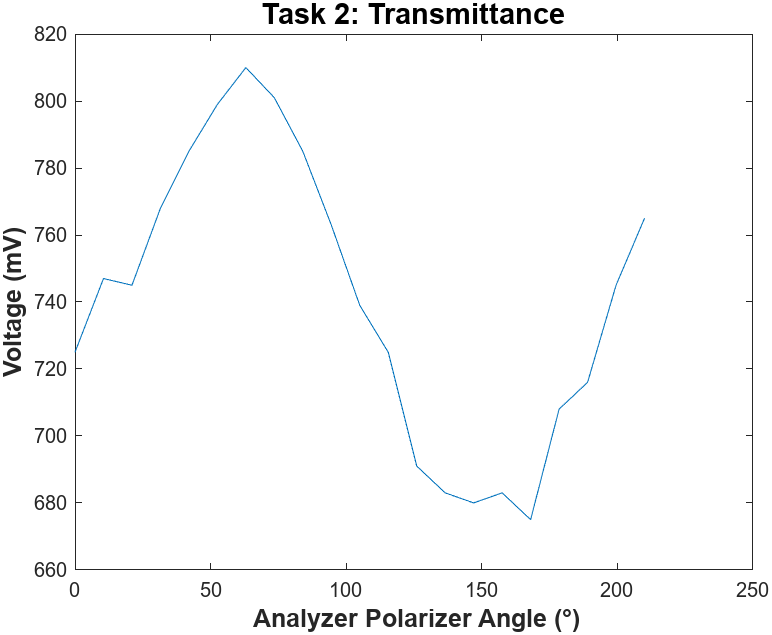
\includegraphics[width=0.35\linewidth]{figs/task2_polar.png}
    \end{subfigure}
    
    \caption{Left: Light intensity dependency on analyzer orientation. Right: Polar plot of the light intensity as a function of the analyzer orientation. A circular plot indicates a orientation independent signal. Our measured angle range was unfortunately less than 360° which makes the plot not be closed.}
    \label{fig:t2}
\end{figure}

 The small angular dependency resembles the one observed previously (see Fig. \ref{XXX}). This suggests that a small component of the light did not get circularly polarized, but rather remained linearly polarized, and it was this component that gets filtered by the analyzer based on its orientation.
 The constant (angle independent) intensity component of the measured signal represent the circularly polarized component of the light, which is not affected by the orientation of the linear analyzer polarizer.
% circular plot


% TASK 3 AND 4

We synthesize a 2kHz rectangular signal and apply it to the LC cell. We measure the voltage deendency of the measured light intensity. 







\subsection{Detection of hemozoin suspended in water}

% TASK 5

In order to measure the second harmonic, we use a lock-in frequency (20Hz) twice as large as the driving frequency (10Hz)

% The results from the lockin measurement were not very precise, and repeated mesurements yielded slightly different results. 

The quality of the calibration curve is limited by the few datapoints available. We were expecting a linear relationship (at least, for not very large concentrations where some saturation is expected), which is difficult to validate given the limited data. The discprenacy seen at the 0\% concentration sample could be accounted for by considering it the baseline effect caused by the elements other than the hemozoid. % XXX improved
Furthermore, there were more bubbles in the 0\% concentration sample. However, linear or nonlinear, a well done calibration curve can be effectively used to calculate the concentration level of hemozoid by interpolation, which makes this technique useful for diagnosis.


% Conclusion
\section{Conclusion}

Manually rotating the polarizer and calibrating the measurement setup introduced some limitations and errors which could be reduced by more precise automatized controls.
We could construct a calibration curve that relates the concentration of hemozoid to the measured optical signal. I would be greatly improved by increasing the number of datapoints used for the curve.

\end{document}